%!TEX TS-program = lualatex
%!TEX encoding   = UTF-8 Unicode

\documentclass[aspectratio=169]{beamer}

\usepackage{tikz}
\usepackage{svg}
\usepackage{subfiles}
\usepackage{hyperref}
\usepackage{hyperxmp}
\usepackage{qrcode}
\usepackage{figures}
\usepackage[export]{adjustbox}

\setlength {\marginparwidth }{2cm}
\hypersetup{
  pdfcopyright = {Copyright (C) 2023 by Krv Analytics.
    All rights reserved. Do not distribute.},
  pdflicenseurl = {http://latex-community.org/license/}}
  
\tikzstyle{box} = [rectangle, rounded corners, minimum width=1.5cm, minimum height=1cm,text centered, draw=black, fill=white]
\tikzstyle{box2} = [rectangle, rounded corners, minimum width=0.5cm, minimum height=0.5cm,text centered, draw=black, fill=white]
\tikzstyle{arrow} = [thick,->,>=stealth]

\usetheme{purus}

%%%%%%%%%%%%%%%%%%%%%%%%%%%%%%%%%%%%%%%%%%%%%%%%%%%%%%%%%%%%%%%%%%%%%%%%
% Title
%%%%%%%%%%%%%%%%%%%%%%%%%%%%%%%%%%%%%%%%%%%%%%%%%%%%%%%%%%%%%%%%%%%%%%%%

% 
\title[Transaction Anomaly Detection]{Identification and Classification of Transaction Anomalies}
\institute{Applying isolation outlier detection and topological profiling to GL Transaction data.}

%%%%%%%%%%%%%%%%%%%%%%%%%%%%%%%%%%%%%%%%%%%%%%%%%%%%%%%%%%%%%%%%%%%%%%%%
% Slides
%%%%%%%%%%%%%%%%%%%%%%%%%%%%%%%%%%%%%%%%%%%%%%%%%%%%%%%%%%%%%%%%%%%%%%%%

\begin{document}
  \begin{frame}[noframenumbering, plain]
    \titlepage
  \end{frame}

\begin{frame}{Some Terminology}
  \begin{itemize}
    \item \textit{Outlier}: an extrememal transaction (ie differeing extensively from a reference set of transactions) 
    \item \textit{Anomaly}: an unexpected pattern of transactions
    \item \textit{Suspect}: a transaction that has been flagged as potentially erroneous or malicious
    \item \textit{Guilty Transaction}: a confirmed erroneous or malicious transaction (and intuitively there also exist innocent suspects).
  \end{itemize}
\end{frame}

\begin{frame}{The Goal}
We split the obvious end of identifying all guilty transactions into two simpler subgoals: 
\begin{enumerate}
  \item Profiling Suspects 
  \item Identifing outliers in target profiles 
\end{enumerate}
Performing these two tasks will generate a case against suspects. Like a competent prosecutor, only convincing cases should 
lead to an accusal. 
\end{frame}
  \begin{frame}{Building a Good Case}
    Sticking with our metaphor, the classic "motive, means, opportunity" evaluation
    will translate to "danger and difference" from a data-driven perspective. 
    \begin{itemize}
      \item \textit{Danger}: contexualized properties that identify erratic, peculiar, 
    unexplained or risky behavior
    \item \textit{Difference}: also to be thought of as distance, refers to the necessary 
    separation between guilty and innocent transactions.      
    \end{itemize}
    
  \end{frame}

  \begin{frame}{Evaluating Anomalies}
    \begin{center}
      \begin{figure}
        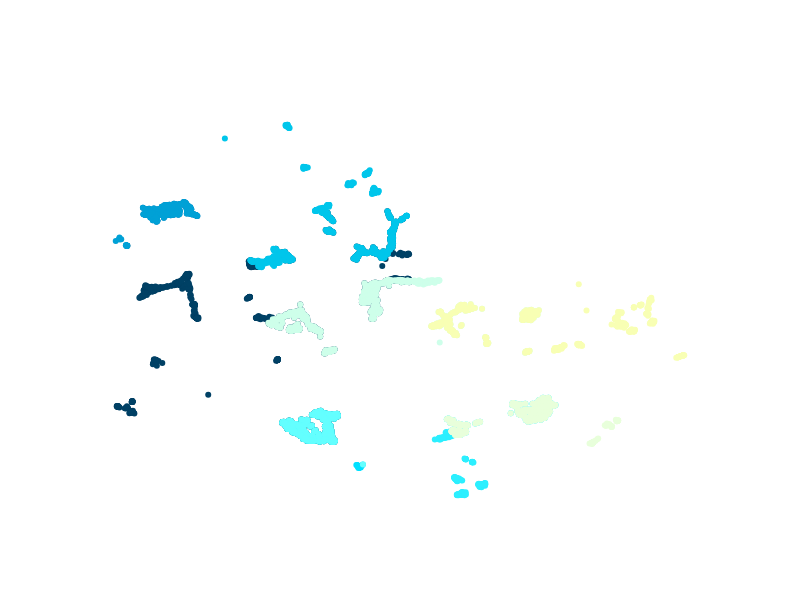
\includegraphics[width=0.5\textwidth]{images/projection.png}
        \label{fig:1}
        \caption{Figure 1: A two dimensional embedding of the suspect list}
      \end{figure}
    \end{center}
  \end{frame}

  \begin{frame}{Evaluating Anomalies}
    \begin{tikzpicture}[overlay, remember picture]
      \node at (current page.north east)
       [anchor=north east, inner sep=0] {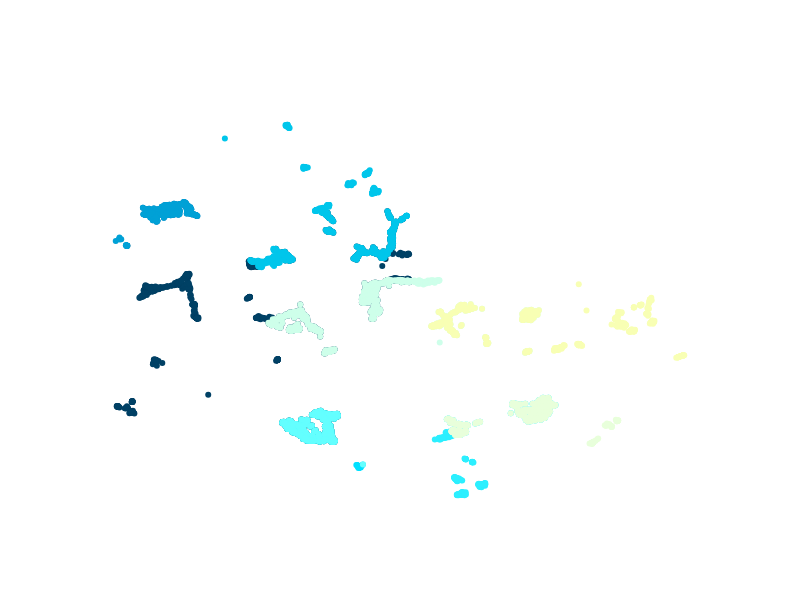
\includegraphics[width=0.4\textwidth]{images/projection.png}};
    \end{tikzpicture} 
    \begin{itemize}
      \item In order to identify \textit{dangerous anomalies}, we must create a reference 
      profile to compare against
      \item We aim to answer the question: "Who are important neighboring transactions that 
      may testify to guilt or innocence?" 
    \end{itemize}
    \end{frame}

  \begin{frame}{Classification using THEMA}
    \begin{center}
      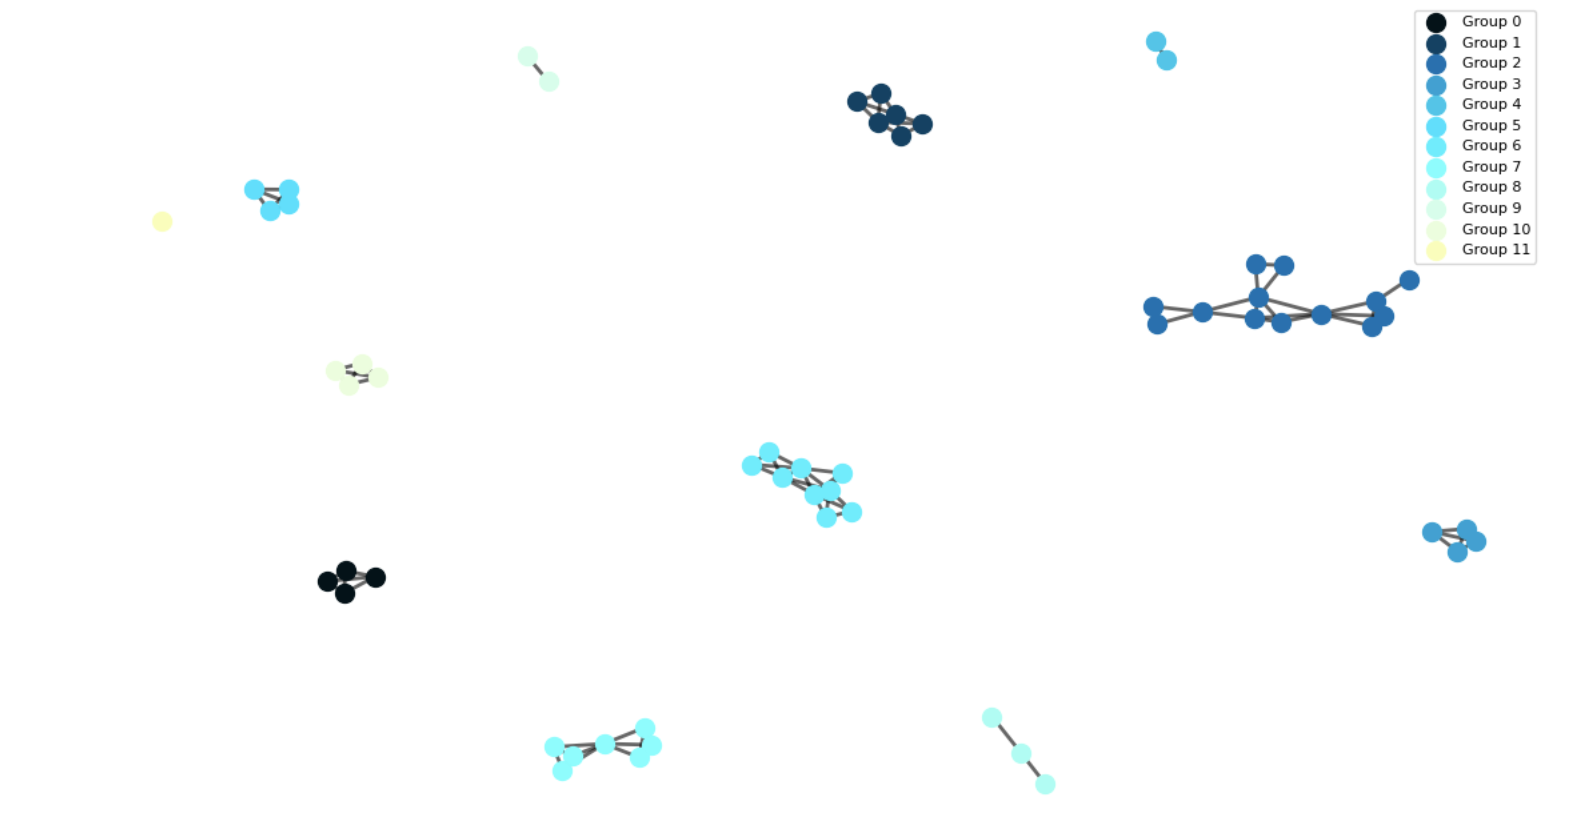
\includegraphics[width=0.9\textwidth]{images/model12.png}
    \end{center}
  \end{frame}

  \begin{frame}{Classification using THEMA}
        \begin{tikzpicture}[overlay, remember picture]
          \node at ($(current page.north east) + (-0.05\textwidth,-0.07\textwidth)$)
           [anchor=north east, inner sep=0] {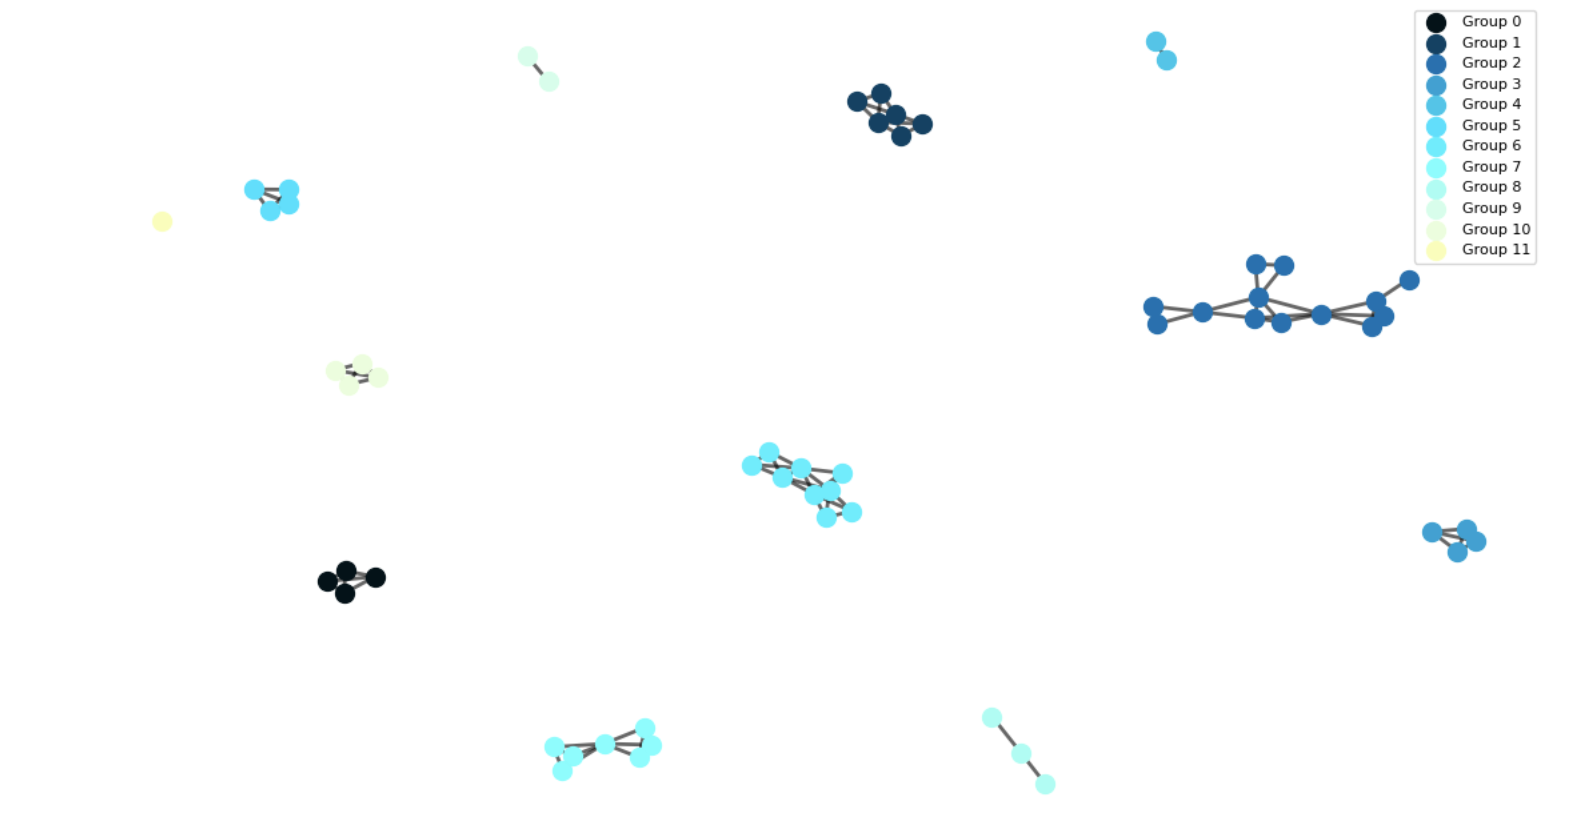
\includegraphics[width=0.4\textwidth]{images/model12.png}};
        \end{tikzpicture}   
        We will associate \textit{danger} with  
        \begin{itemize}
          \item Inconsistencies in a group across a relevant attribute   
          \item Small, localized and highly homogenous groups  
        \end{itemize}
        The idea behind these two methods is to flag both singleton suspects and families of suspects based 
        on thier group profiles. A group profile itself may be \textit{dangerous} or it 
        may provide a reference point for establishing danger.
        \end{frame}



  \begin{frame}{Establishing Difference}
    We generate a suspect list by identifying outliers in our group profiles. These suspects can be thought 
    of as misfits of a groups normalcy, and as such possess inherent \textit{differences} from their peer group.
    To do this, we construct Isolation Forests that
    \begin{itemize}
      \item identify transactions with signifcant difference from its groups global norm
      \item ignore highly regular, indistinguishable transactions 
    \end{itemize}
    Note: There may exist guilty transactions who are considered inliers for a particular "problematic" group. The hope 
    is that a group's profile itself will be flagged. 
  \end{frame}

  \begin{frame}{Isolation Forests}
    \begin{columns}
      \begin{column}{0.5\textwidth}
        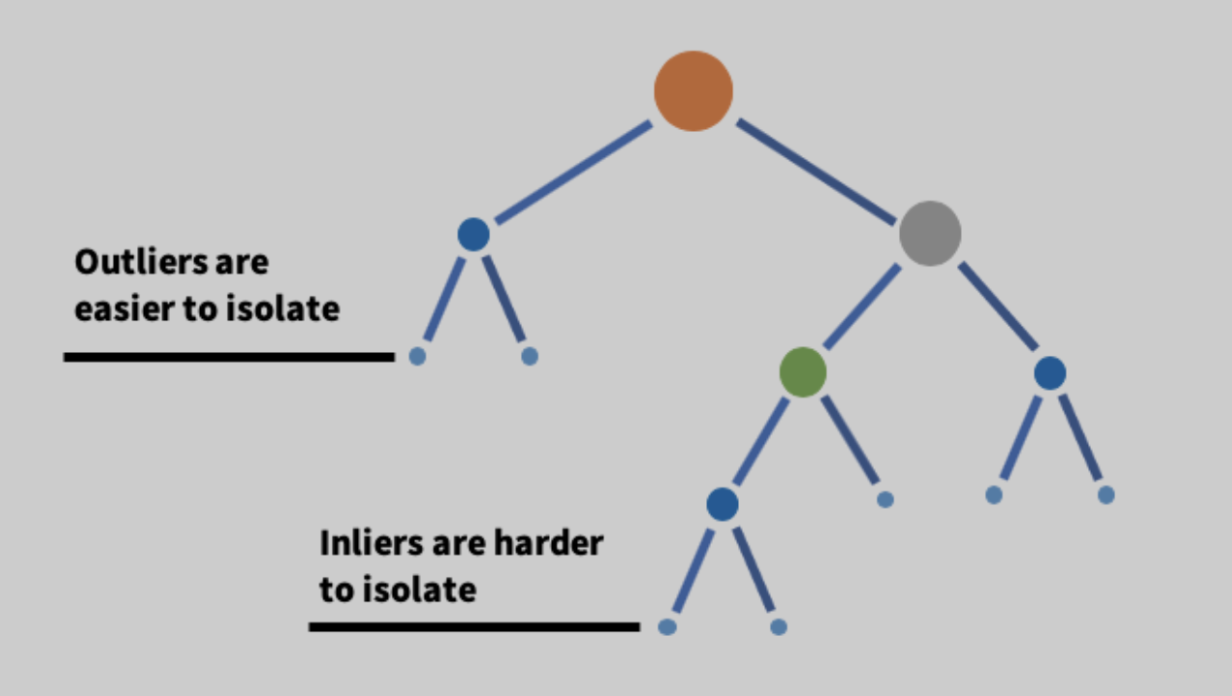
\includegraphics[width=\textwidth]{images/iso_forest.png}
      \end{column}
      \begin{column}{0.5\textwidth}
        \begin{itemize}
          \item train a model to recognize isolated patterns within a profile
          \item outliers isolated due to unexpected behavior are labelled as \textit{dangerous}
        \end{itemize}
        \textbf{Remark} Assuming guilty transactions must have some point of difference does not 
        imply that severe outliers are better suspects.
      \end{column}
    \end{columns}  
  \end{frame}

  \begin{frame}{Results}
    \begin{itemize}
      \item Beginning with a dataset of 31,970 transactions, we present following 17 transactions 
      as a suspect list 
      \item This list was built with no prior knowledge of transaction types or account information.
      \item For the complete suspect list, please consult the associated data file. 
      \item After constructing an initial list, we create a list targetting anomolous cash account transactions. 
    \end{itemize}
  \end{frame}

  \begin{frame}{Results}
    \begin{center}
    \resizebox{\linewidth}{!}{
    \begin{tabular}{|c|c|c|c|c|c|}
      \hline 
      \textbf{ID} & \textbf{JE Doc Type} & \textbf{G/L Accounts} & \textbf{Cost Center} & \textbf{Profit Center} & \textbf{Assignment Reference} \\\hline
      510014000013232023  & Customer payment    & \{110000, 104011\}                            & {n/a}	        & {AbbVie}	                 & {20230103, n/a} \\\hline
      51001000471862020   & HR Payroll Entries  & 	\{230050, 104011, 230060, 600530, 230070\}  & {n/a, 51043}	& {Overheads}	               & {Payroll Liabilitie}\\\hline
      51001000502952021   & Concur Exp. Posting & \{110010, 104011\}                            & {n/a}	        & {Madiba General}	         & {20210326, Amex March 2021}\\\hline
      510014000013982023  & Customer payment	  & \{110000, 520130, 104012\}                    & {n/a}         & 	{AbbVie (House), AbbVie} & {20230207, n/a}\\\hline
      510014000014582023  & Customer payment    & \{110000, 104012\}                            & {n/a}         & {Madiba General}	         & {n/a, 20230309}\\\hline
      510014000013982023  & Customer payment    & \{110000, 520130, 104012\}                    & {n/a}         & {AbbVie (House), AbbVie}	 & {20230207, n/a}\\\hline
      510014000013232023  &  Customer payment   & \{110000, 104011\}	                          & {n/a}	        & {AbbVie}	                 & {20230103, n/a}\\\hline
    \end{tabular}
    }
  \end{center}
  \end{frame}

\end{document}
